\subsection{Motivating Example}
\label{motivatingExample}

As a motivating example, we consider the problem of autonomous flight of a hexrotor along a pre-defined pattern.
A hexrotor is a flying robot with six rotating blades.[???]
It carries a downward facing camera that sees salient features of the environment.
See Fig.~\ref{fig:hexrotor}.
\begin{figure}[htp]
	\centering
	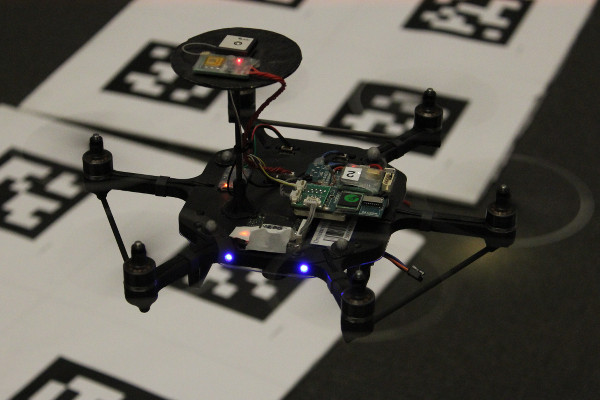
\includegraphics[width=0.9\columnwidth]{figures/nanohex}
	\caption{Hexrotor flying over synthetic features}
	\label{fig:hexrotor}
\end{figure}
These are detected by an on-board corner detector, and tracked by a visual odometry algorithm in order to estimate the robot's position in the world.
After each frame is acquired, the visual odometry algorithm requires some computation time before producing its results, which are used in self-localization.
Thus the control command which uses this estimate is delayed by the time necessary to run the estimation task to completion.
This is illustrated in Fig.~\ref{fig:senseActuate}.
\begin{figure}[t]
	\centering
	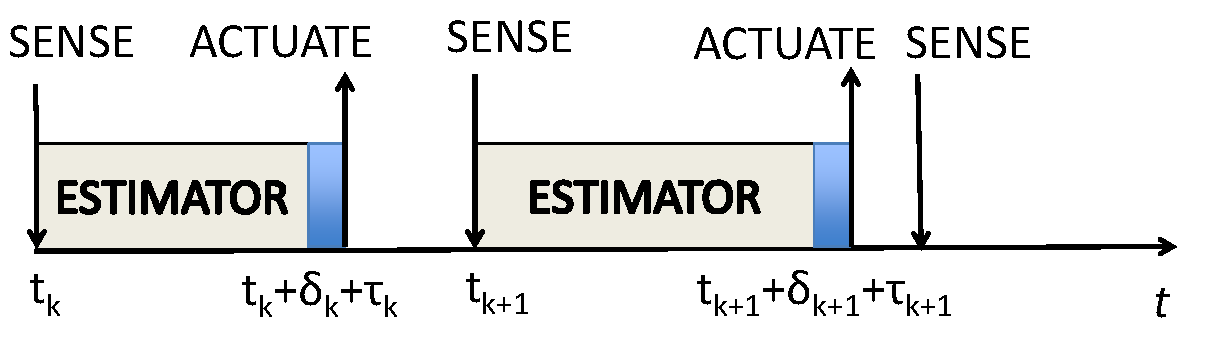
\includegraphics[width=0.9\columnwidth]{figures/senseActuate}
	\caption{Sense-Estimate-Actuate cycle. The estimation task always runs to completion.}
	\label{fig:senseActuate}
\end{figure}
The robot has a high-level controller which determines the desired pitch and roll angles, and desired rotor thrust.
In this implementation, we use a Model Predictive Controller (MPC) [???].
As the robot is commanded to fly the pattern faster and faster, the estimator delay affects the control performance more.
\todo[inline]{Pending experimental confirmation about the effect of speed of flight on control performance }
The control performance, as measured by a function that factors in the error in following the flight path and the cost of control, is shown in Fig.~\ref{fig:degradingPerformance}.
(The details of this cost function are given in Section \ref{formulation}).

Running an estimation task with a fixed smaller delay but larger estimation error does not necessarily solve the problem of degraded performance.

Therefore, there is a need to rigorously quantify the trade-off between computation time and estimation error, then exploit that trade-off intelligently to achieve the best control performance under the problem constraints.
Rather than always run the estimation task to completion, it is useful to have several estimation tasks with varying utilities (i.e., varying delay/error trade-offs).
These can then be used at runtime to satisfy the control objectives.
